\section{Pengertian Web Hosting}
\hfill \break
Web Hosting adalah sebuah komputer yang terhubung ke internet dan dipergunakan untuk menyimpan data website agar dapat diakses secara online. 
\hfill \break
Dengan memakai web hosting ini maka seluruh informasi yang disimpan dapat ditampilkan.Semua informasi yang disimpan di sebuat tempat disebut server web hosting. Untuk bisa tersabung ke internet dan dapat diakses oleh semua orang, server web hosting dikelola dalam ruang penyimpanan data bernama daat center.
\hfill \break
Istiah web hosting sendiri merujuk pada set aktivitas atau layanan penyimpanan informasi sautu website hingga akhirnya bisa ditampilkan ketika Anda akses. 

\section{Cara Kerja Web Hosting}
\hfill \break
\begin{figure}[!htbp]
  		 \centering
 		 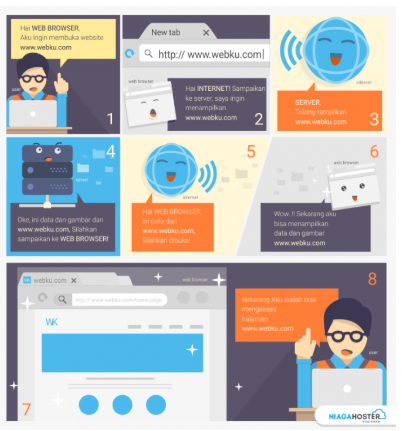
\includegraphics[width=.75\textwidth]{figures/web.png}
  		 \caption{Cara Kera web hosting}\label{fig:done}
		 \end{figure}
\hfill \break
Ketika teman-teman ingin mengases suatu website, maka teman-teman perku mengetikkan alamat website pada browser yang teman-teman gunakan.
\hfill \break
Kemudian, browser akan mengeksekusi perintah yang akan diteruskan dari internet ke server hosting sesuai permintaan. Hasil nya yaitu akan menampilkan gambar dan informasi website sesuai yang di akses dan akan diteruskan oleh internet agar tampil pada browser teman-teman. Jadi, begitulah cara kerja web hosting.
